\documentclass[11pt]{article} %Sets the default text size to 11pt and class to article.
\usepackage{amsmath,amsfonts,amssymb,verbatim}
\usepackage{graphicx}
\newcommand{\BigO}[1]{\ensuremath{\operatorname{O}\bigl(#1\bigr)}}

%------------------------Dimensions--------------------------------------------
\topmargin=-.5in %length of margin at the top of the page (1 inch added by default)
\oddsidemargin=-0.2in %length of margin on sides for odd pages
\evensidemargin=0in %length of margin on sides for even pages
\textwidth=6.5in %How wide you want your text to be
\marginparwidth=0.5in
\headheight=0pt %1in margins at top and bottom (1 inch is added to this value by default)
\headsep=0pt %Increase to increase white space in between headers and the top of the page
\textheight=10.0in %How tall the text body is allowed to be on each page
\pagestyle{empty}
\begin{document}
\centerline{{ \LARGE \bf Problem Set 8}} 
\centerline{CSCI 3104 $\bullet$ Spring 2014 $\bullet$ Birthday: 07/22} 
\centerline{Cristobal Salazar}
\centerline{Partner: Alex Tsankov}
\line (1,0){470}
\\
\\
\noindent{\Large \bf Problem 1}
\\
\\
\noindent{ \large a) See Fig. 1 below. T = tree edge, B = back edge, F = forward edge, and C = cross edge. We are assuming DFS begins with vertex 1. 
\\
\begin{figure}[ht!]
\centering
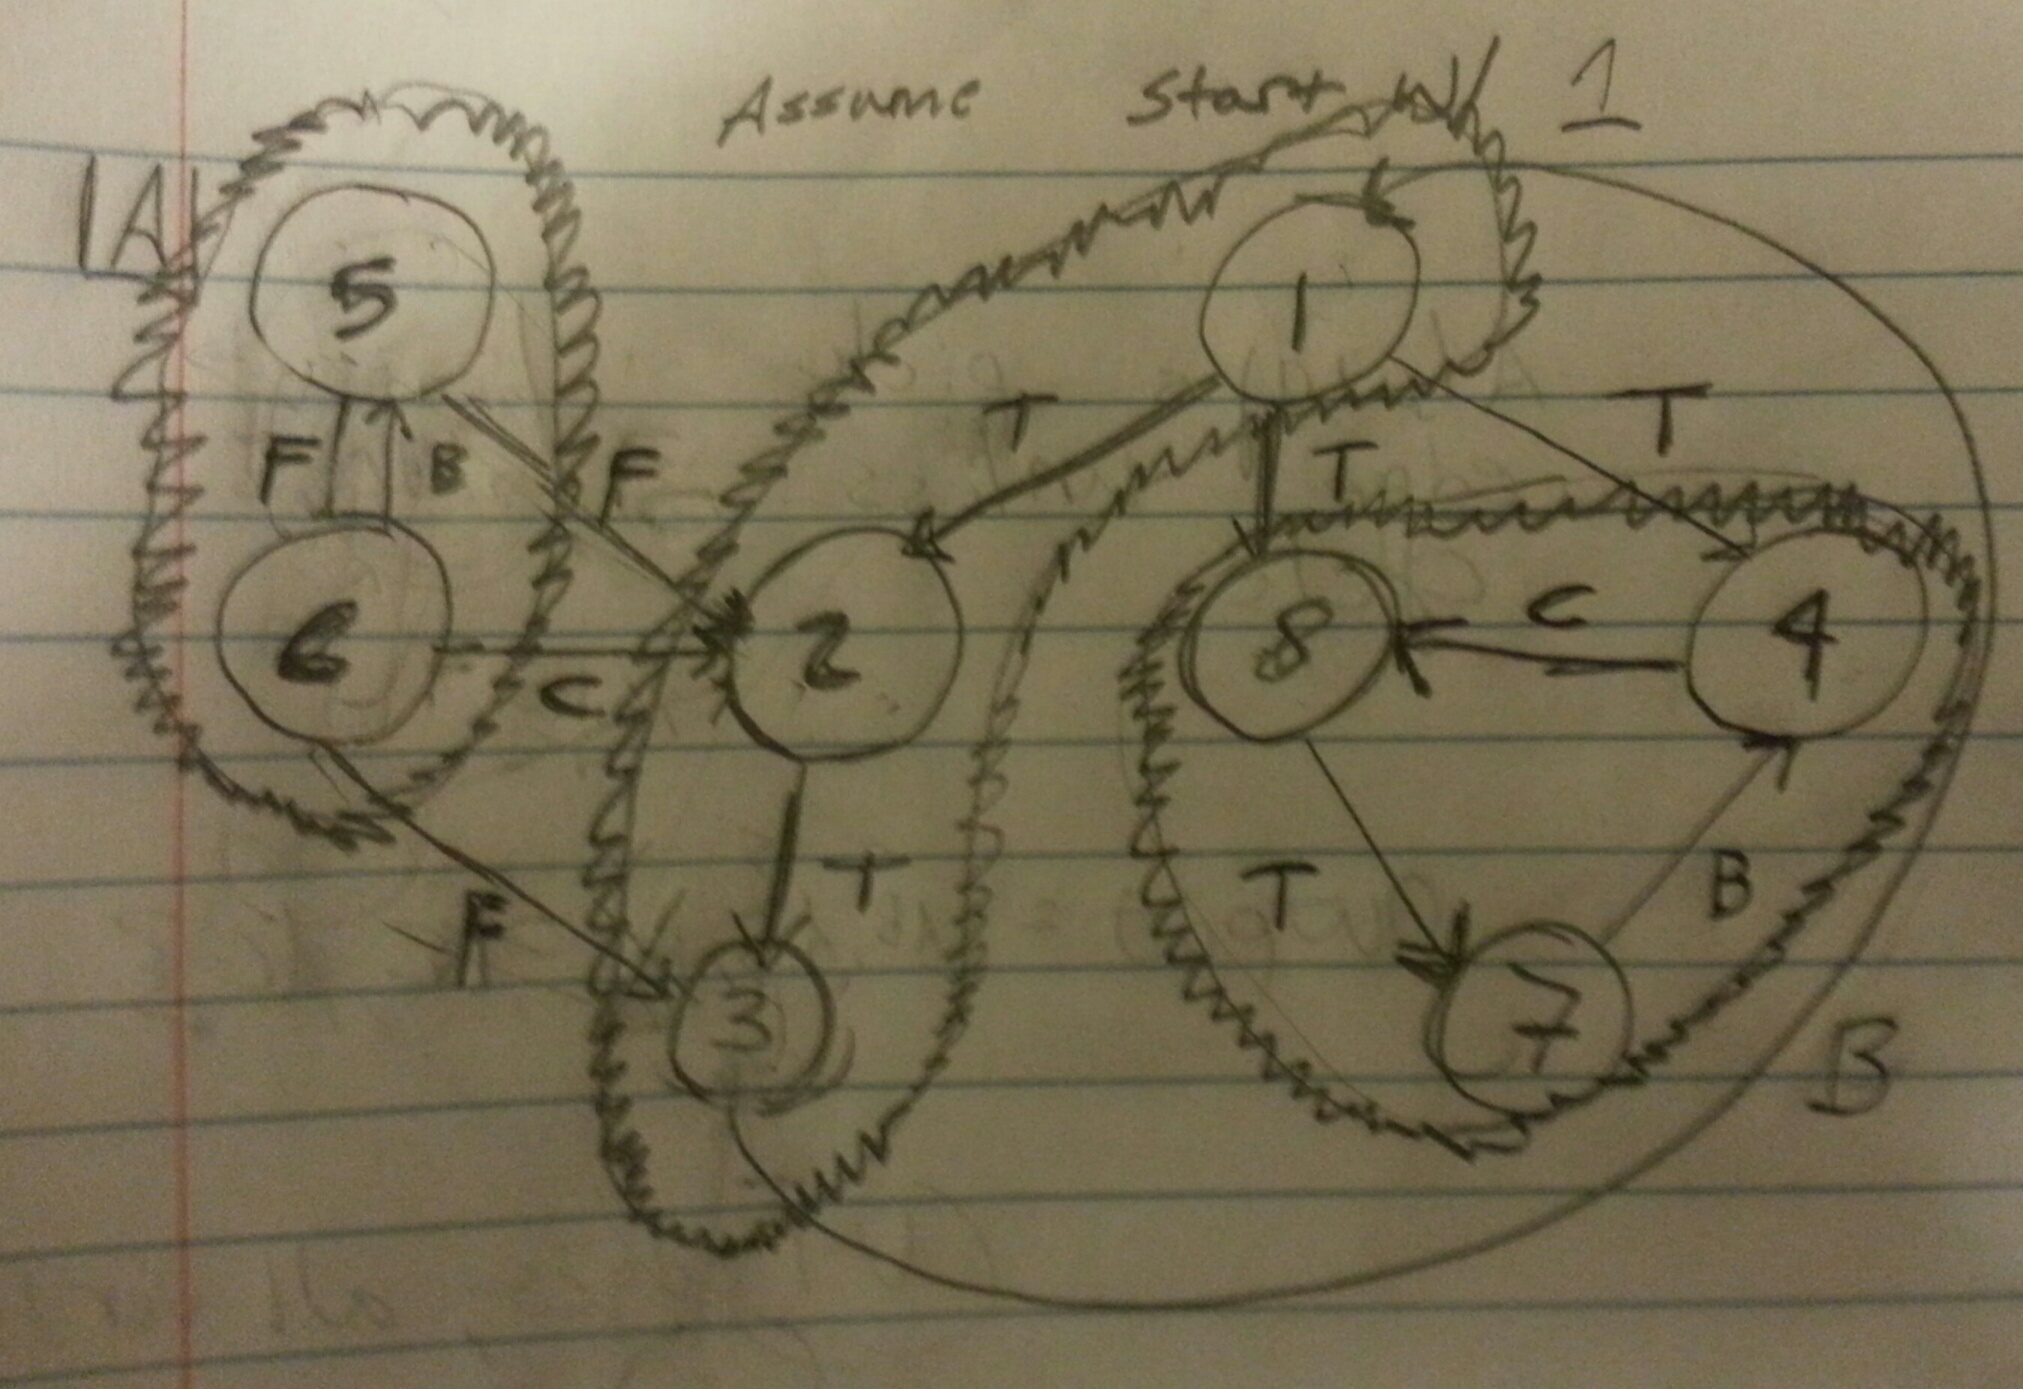
\includegraphics[width=150mm]{prob_1a.jpg}
\caption{Tree made from edge set with labelled directed edges}
\label{overflow}
\end{figure}
\\
\noindent{ \large b) Strong components are as follows: $[8,4,7],[1,2,3],[5,6]$. See grouped nodes in Fig. 1 for a visualization of the strong components.} 
\\
\\
\noindent{\Large \bf Problem 2}
\\
\begin{figure}[ht!]
\centering
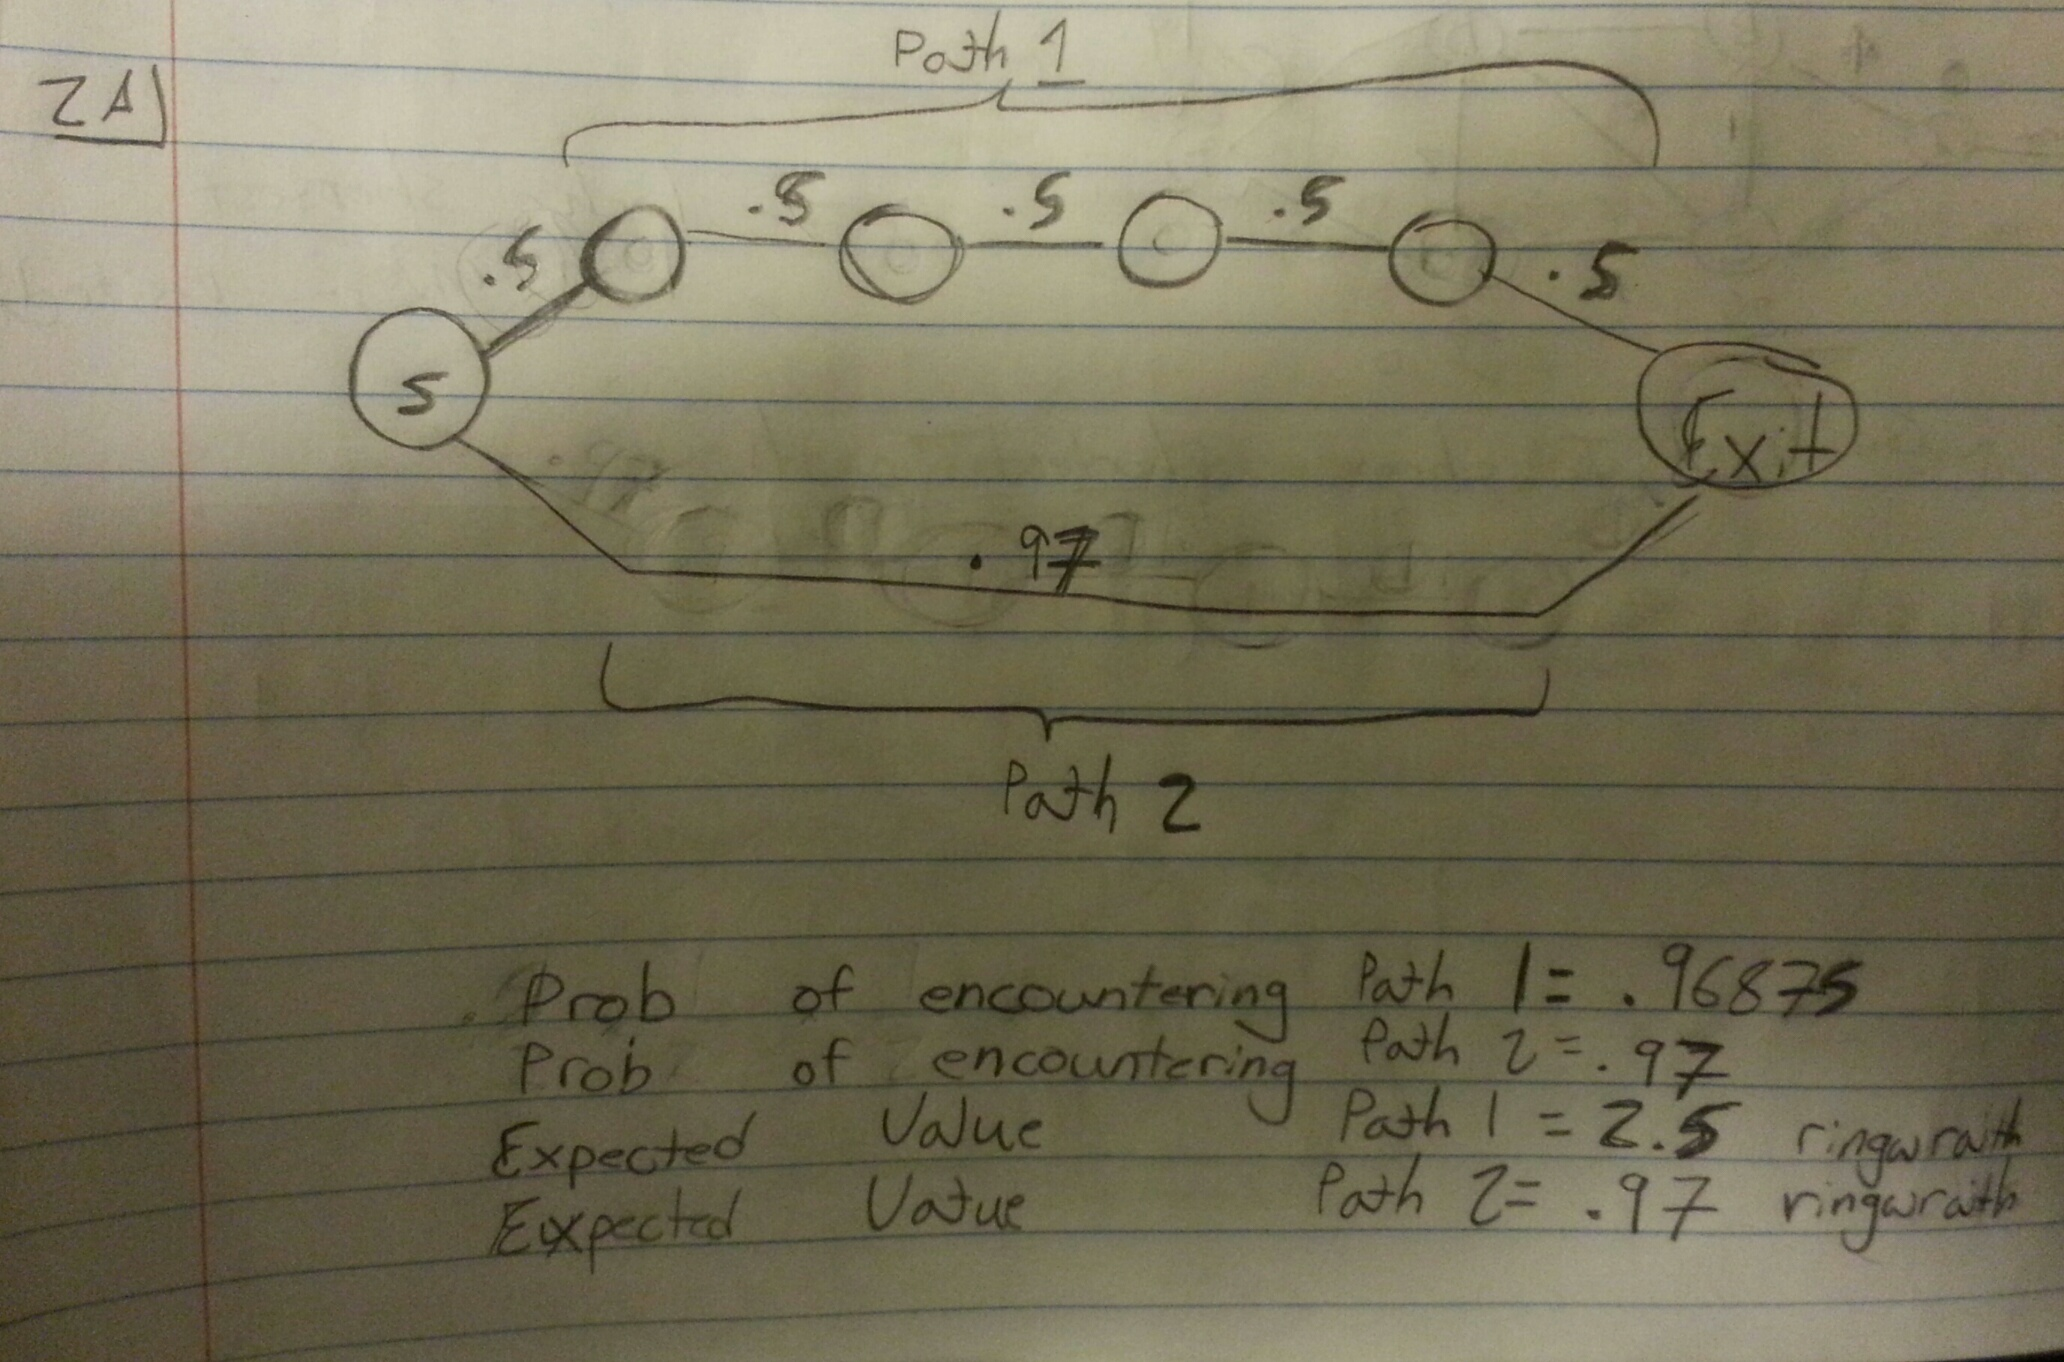
\includegraphics[width=150mm]{prob_2a.jpg}
\caption{Tree made from edge set with labeled directed edges}
\label{overflow}
\end{figure}
\\
\noindent{\large a) See Fig. 2 for a visualization of the graph. If we take Path 1, our probability, $P_1$, of encountering a ringwraith is .96875. We reached this number by subtracting the combined likelihood of not encountering a ringwraith on Path 1, $(\frac{1}{2}*\frac{1}{2}*\frac{1}{2}*\frac{1}{2}*\frac{1}{2})$ or $.03125 $ from 1, which gives us a $P_1$ $= .96875$. The $P_2$ for Path 2 is simply $.97*1$, a .97 percent chance of encountering a ringwraith. Therefore, if we hope to minimize our probability for encountering a ringwraith, Path 1 would be better.
\\
\\
\noindent{\large However, if we calculate the expected value, $E_1$, of Path 1, which we can do by calculating probability of encountering a monster on each edge multiplied by 1, and eventually adding the total $(\frac{1}{2}*1 + \frac{1}{2}*1 + \frac{1}{2}*1 + \frac{1}{2}*1 + \frac{1}{2}*1),$ or $2.5$. The $E_2$ value of Path 2 is $(.97*1)$, or $.97$. The path with the lower $E$ is Path 2.   
\\
\\
\noindent{\large b) To find the path with the lowest possible expected value or $EV$ of encountering ringwraiths, we can use Dijkstra's algorithm (DA) on a modified graph. \\\\ Step 1) We begin by splitting every edge and creating a directed graph. We calculate the weight for these two new edges, for example (u,v) and (v,u) by taking the previous edge weight, (u,v), and adding it to the weight of the vertex $W(u,v) = P(u) + P(u,v)$ and $W(v,u) = P(v) + P(u,v)$ .  This takes $O(2E)$ time, two calculations for each newly-split edge. \\Step 2) Run DA on the modified paths to find the SSSP. This takes $O(E + V lg(V))$\\If we put together Step 1 and Step 2, we have a total run time of $O(E + V lg(V) + 2E)$  }
\\
\\
\noindent{\large c)To find the path with the lowest possible probability or $P$ of encountering  ringwraiths, we can use DA on a modified graph. \\\\ Step 1) We begin by splitting every edge and creating a directed graph. We calculate the weight for these two edges, in our case (u,v) and (v,u) by taking the previous edge weight and multiplying it by the negative logarithm of the probability of the vertex. For example, $W(u,v) = -log(P(u) * P(u,v))$ and $W(v,u) = log(P(v) * P(u,v)$. By using logarithms we avoid negative path weights that would break DA. This takes $O(2E)$ time, like the problem above. \\Step 2) Run DA on the modified paths to find the SSSP. This takes $O(E + V lg(V))$\\If we put together Step 1 and Step 2, we have a total run time of $O(E + V lg(V) + 2E)$}
\\
\\
\noindent{\Large \bf Problem 3}
\\
\indent{\large a) If we have a graph G with four vertices:\{A, B, C, D\}, with weighted edges:\{AB:1, AC:12, BC: 1, CD: 2\}, we will have a unique minimum spanning tree. This graph has the following two spanning trees from vertex A with edges: $T_1=$\{AB:1, BC:1, CD:2\} and $T_2=$\{AB:1,AC:12,CD:2\}. Even though there are two spanning trees, there is only one, unique MST ($T_1$).}
\\

\indent{\large b) For this problem, we must assume that edge weights do not have to be distinct. If all edge weights are distinct, then Golum would be correct. So, assuming we can have multiple edges with the same weight, the following undirected graph $G$ has two MSTs: \\vertices:\{A, B, C, D, E, F\}\\edges:\{AE:2, AB:4, BC:4, BD:4, DC:4, CF:2\} \\We can see that no edge is unique, and there is still two minimum spanning trees, therefore Golum's claim is incorrect.See Figure 3 for an illustration of this.}
\\
\\
\begin{figure}[!htb]
\centering
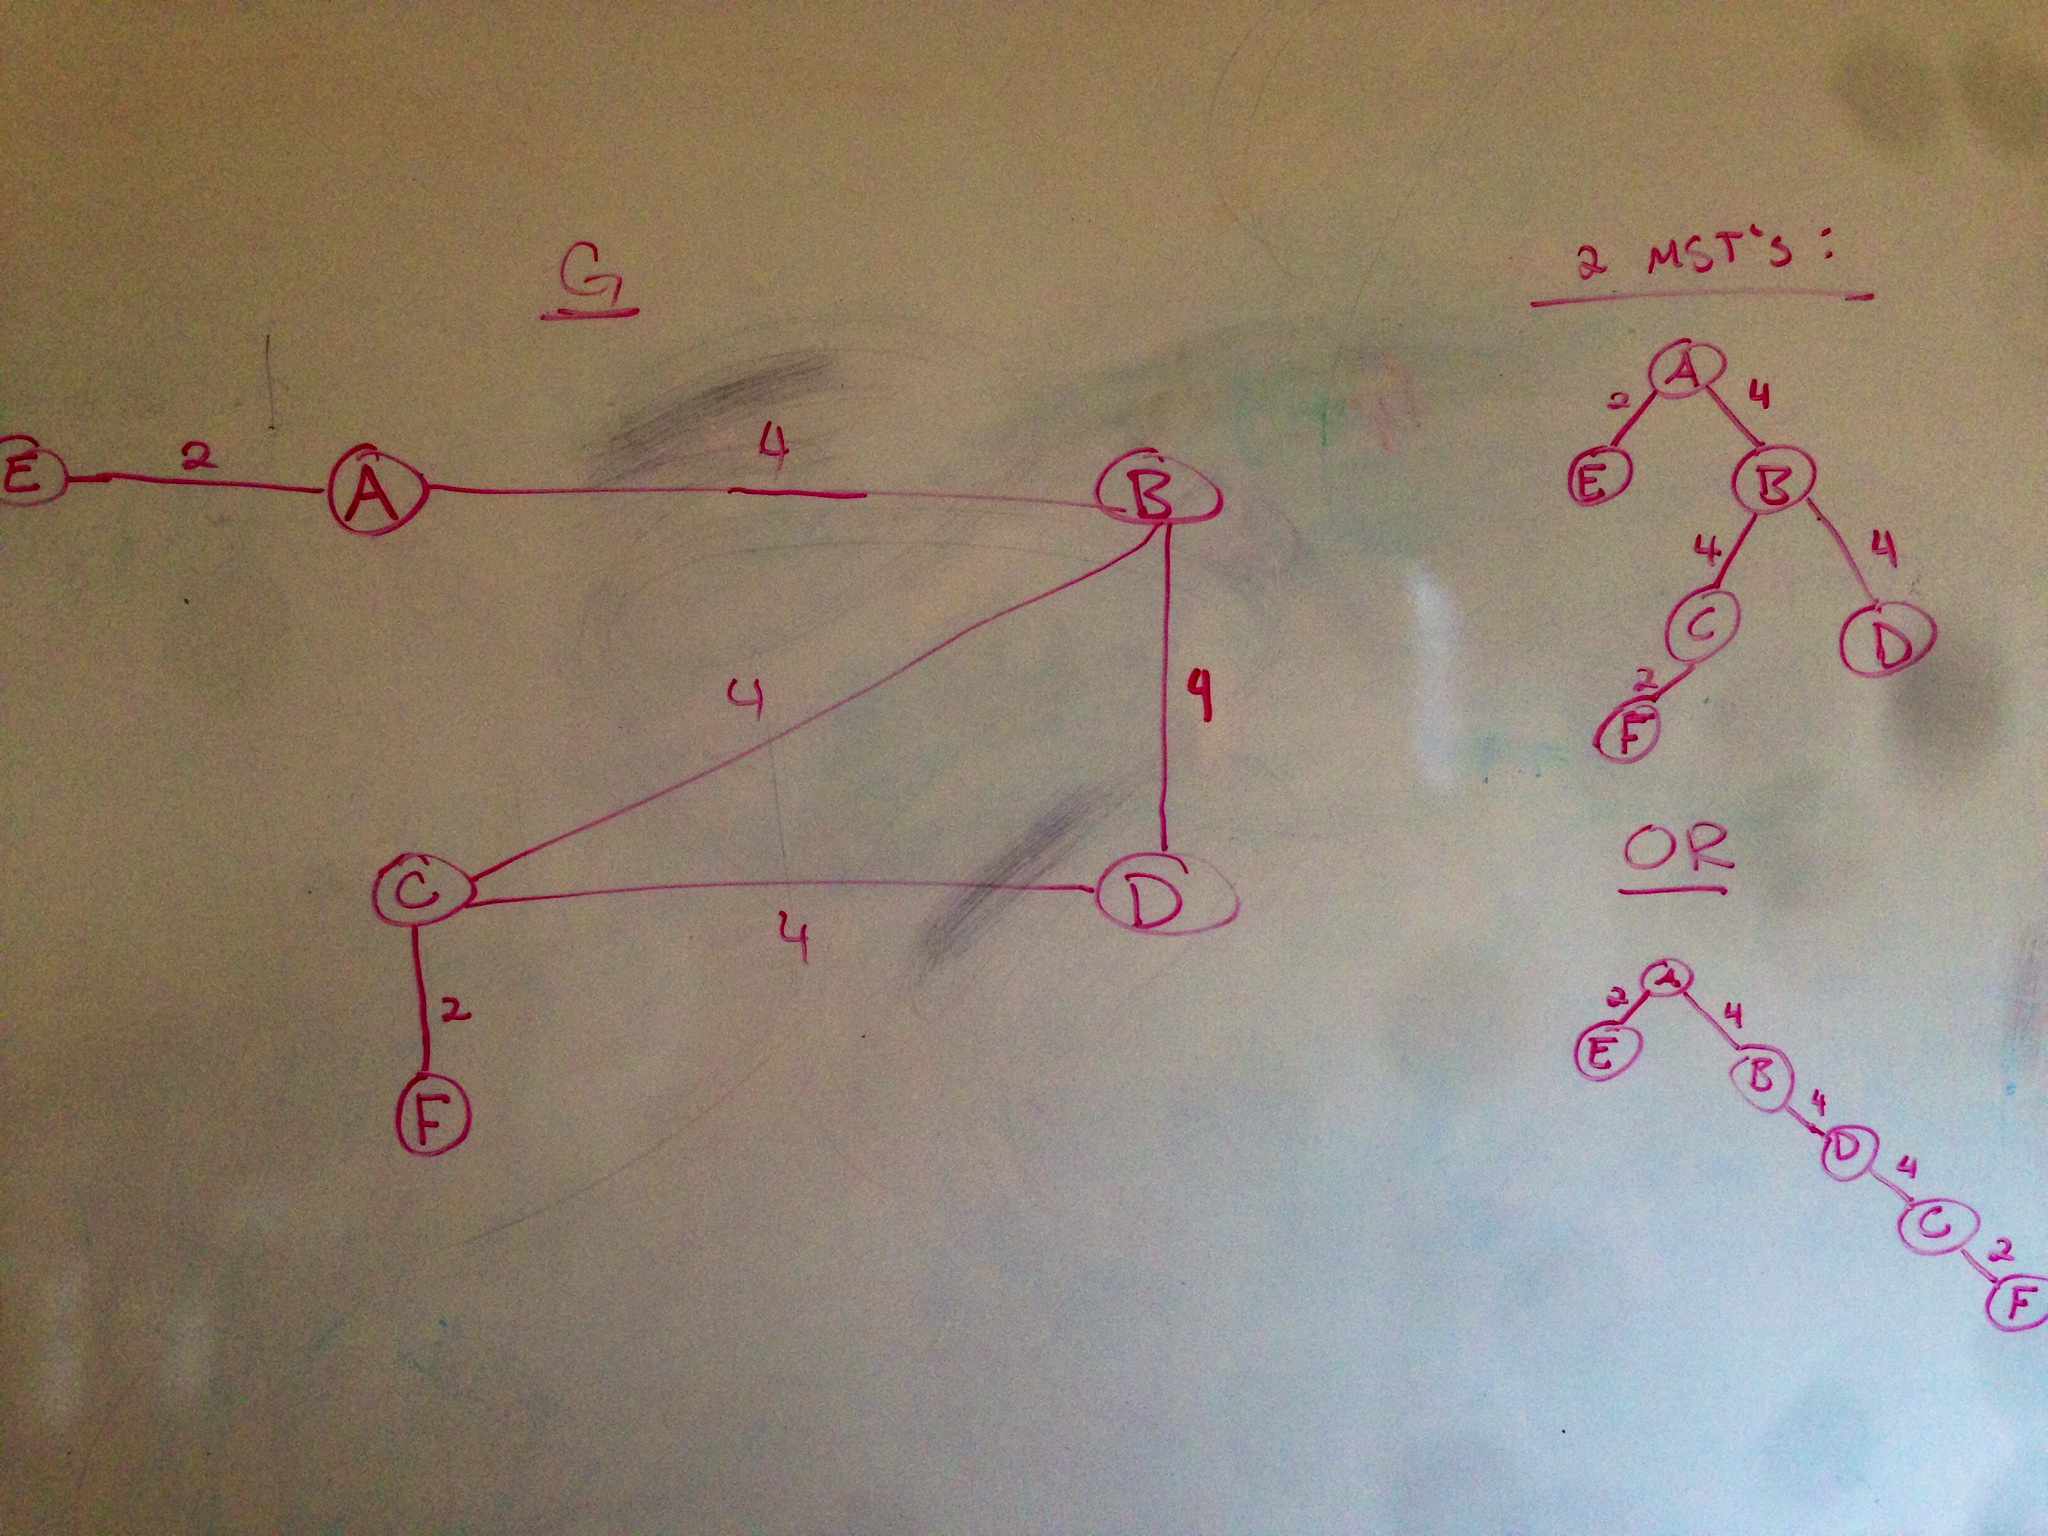
\includegraphics[width=160mm]{prob_3b.JPG}
\caption{Run time of our Dijkstra's Algorithm}
\label{overflow}
\end{figure}
\\
\\
\indent{\large c) For this claim, we must assume that edge weights do not have to be distinct. To prove the claim by contradiction we say that graph $G$ has two minimum spanning trees, $T_{MST}$ and $T'_{MST}$. Let edge $(u,v)$ be in the minimum spanning tree $T_{MST}$, but not $T'_{MST}$. If we were to remove the edge from $T_{MST}$, we will cut the tree into two partitions, $T_u$ and $T_v$. Next, let the edge $(a,b)$ be the unique minimum edge crossing the partition. Given $(x,y) \neq (u,v)$ and we know the weight of $(a,b)$$<$ the weight of $(u,v)$, therefore the spanning tree $(T_{MST}-(u,v))\cup(a,b)$ has a less weight than $T_{MST}$, which is a contradiction. Now, since the edge $(u,v)$ is not in $T'_{MST}$, we say that the path between $u$ and $v$ is path $l$.  Because path $l$ exists, we know that there is some edge, $e$, between $T'_u$ and $T'_v$ (A partition of $T'_{MST}$ where $u$ is in $T'_u$ and $v$ is  in$T'_v$). Now, we also know that $W(u,v)<W(e)$ because as stated above, $(u,v)$ is an unique minimum weighted edge. If we add $(u,v)$ to $T'_{MST}$ we get a cycle composed of the edge $(u,v)$ and the path $l$. By removing any edge from the cycle we get the
spanning tree $(T′_{MST} \cup (u,v)) − e$ which has a lower weight than $T′_{MST}$, this is also a contradiction. Therefore we know that given our claim, there can only be one, unique minimum spanning tree.}
\\

\indent{\large d) To do this, we will modify Kruskal's algorithm which takes $O(E*lg(V))$. We can take Kruskal's, and add some checks in the pseudo-code algorithm shown below, to confirm our analysis in part 3C: 
\begin{verbatim}
uniqueMST(G){ 
  int x[] = sortEdges(G) //array of sorted edges
  tree MST = initialize tree
  boolean uniqueCycle = false
  boolean uniqueMinPart = false
  for(i=1; i < x.length; i++){
    if(createsCycle(MST, x[i])){
      if(isMaxUniqueEdge(x[i]))
        uniqueCycle = true
    }
    else{
      addToTree(x[i])
      if(isMinEdgeConnectingPartitions(MST, x[i]))
        uniqueMinPart = true
    }
  }
  if(uniqueCycle && uniqueMinPart)
    return true
  else
    return false
}
\end{verbatim}
This algorithm performs Kruskal's algorithm, while checking to see if our claim from above is satisfied, thus returning true if there is only one, unique MST.
}
\\
\\
\noindent{\Large \bf Problem 4}
\\
\\
\indent{\large Below is our version of Dijkstra's algorithm coded up in Python: }
\\
\begin{verbatim}
########################################################
################Dijkstra's Algorithm###################
########################################################


def dj_shortest_path(G, start, end):
   def flatten(L):       # this flattens our linked list 
      while len(L) > 0: #while our length of linked list is greater than 0: 
         yield L[0]
         L = L[1] #append the rest of our list.

   q = [(0, start, ())]  # This makes a heap with: cost, path_head, rest of path .
   visited = set()       # Visited vertices.
   while True:
      (cost, v1, path) = heapq.heappop(q) #pop the path off of the top of the heap 
      if v1 not in visited:
         visited.add(v1)
         if v1 == end: #if we are at the end 
            return list(flatten(path))[::-1] + [v1] 
            #return a list flattened with the destination 
         path = (v1, path)
         for (v2, cost2) in G[v1].iteritems():
            if v2 not in visited:
               heapq.heappush(q, (cost + cost2, v2, path))

test_g = {'s':{'u':30, 'x':5},
     'u':{'v':1, 'x':15},
     'v':{'y':4},
     'x':{'u':3, 'v':1, 'y':2},
     'y':{'s':7, 'v':6}}

print dj_shortest_path(test_g,'s','y')

#result from test case: ['s', 'x', 'y']
\end{verbatim}
\indent{\large We then ran analysis on the algorithm by generating random Erdos-Renyi graphs and measuring the time it takes for the algorithm to path-find between two random vertices in this graph.For each number of nodes in the graph, we ran the test 20 times and averaged these run times together. Each red dot on the graph represents the average run time for 20 tests (y-axis) on each unique number of nodes (x-axis). For readability, we made the x-axis a logarithmic scale. See Fig. 4 for the actual graph.}
\\
\begin{figure}[!htb]
\centering
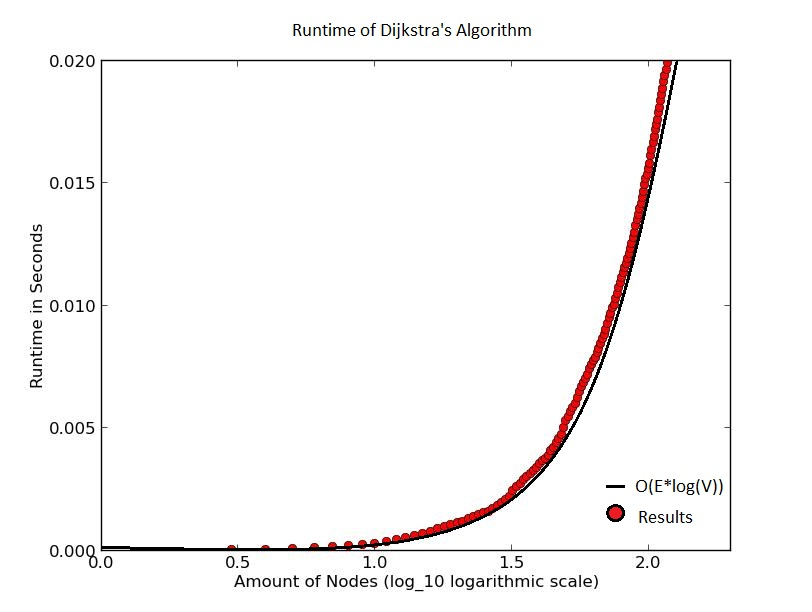
\includegraphics[width=160mm]{prob_4.jpeg}
\caption{Run time of our Dijkstra's Algorithm}
\label{overflow}
\end{figure}
\\
\clearpage
\noindent{\Large \bf Problem 5}
\\
\indent{\large a) To find an arbitrage opportunity, we will need to set up a graph $G$ with vertices representing currencies, and edges representing exchange rates. We must then find a cycle that when multiplying all the edges in the cycle, the product is greater than $1$. We also know that by taking the $log$ of a number, we can add them up and use that to find an increasing cycle. Finally, we can make the $log$ of the number negative to try and find a negative cycle, which is what Bellman-Ford's algorithm does. So, by adding up the $-log$ of all the edges in a cycle and seeing if the sum is negative, we can find an arbitrage opportunity. Also, we can multiply each exchange rate by $1.01,$ for $\alpha=.01$ to account for transaction costs. The algorithm will have the general form:
\begin{verbatim}
arbitrageOp(G, alpha){ 
  Graph allOPs[] = new list of Graphs //put Cycles with neg weight in here
  for(all edges (e) in G){
    e = -log(e)*alpha                //apply changes to every edge
  }
  for(int i = 1;i < vertices.length;i++){ //loop through all vertices
    Graph x = bellmanFord(G, i) //run Bellman-Ford on G with start node i, return cycle
    int sum = findSum(x)    //find sum of weights in cycle x      
    if(sum < 0)
      allOps.add(x) //add the cycle to the list if negative weighted
  }
  return allOps
}
\end{verbatim}
This algorithm has a running time of $O(n^3)$. 
}
\\
\\
\indent{\large b) The algorithm implemented above will give us a list of all possible arbitrage opportunities starting from one currency, and looping around to create a cycle, and ending up at the same currency. The transaction costs, $\alpha$, play a role as to whether or not a cycle is negatively weighted. By multiplying each edge by $1.01$, for $\alpha=.01$  will this take into account the transaction costs. The higher $\alpha$, the less the negative weight of the cycle without transaction costs has to be. So, the greater $\alpha$ gets, the smaller the list of arbitrage opportunities will become, because the cut off of how negative the cycle has to be becomes even less(i.e. more negative). }
\\
\\
\noindent{ \Large \bf Sources}
\\
\noindent{$\bullet$ http://homepages.math.uic.edu/~leon/cs-mcs401-s08/handouts/mst.pdf}
%USE THIS FOR PART 3%
\\
\noindent{$\bullet$ http://en.wikipedia.org/wiki/Bellman%E2%80%93Ford_algorithm#Algorithm}
\\
\noindent{$\bullet$ http://math.stackexchange.com/questions/94414/an-algorithm-for-arbitrage-in-currency-exchange}
\\
\noindent{$\bullet$http://code.activestate.com/recipes/119466-dijkstras-algorithm-for-shortest-paths/}
\\
\end{document}